Calcula el valor de $x$ en el triángulo isóseles  que se muestra abajo (figura \ref{fig:findangle01}).

\begin{minipage}[t][][t]{0.35\textwidth}
    \begin{figure}[H]
        \centering
        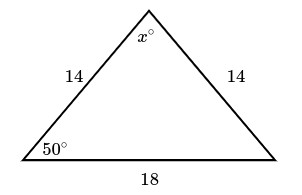
\includegraphics[width=0.9\linewidth]{../images/findangle01.png}
        \caption{}
        \label{fig:findangle01}
    \end{figure}
\end{minipage}\hfill
\begin{minipage}[t][][t]{0.6\textwidth}
    \begin{solutionbox}{8cm}
        \begin{minipage}{0.3\textwidth}
            \begin{figure}[H]
                \centering
                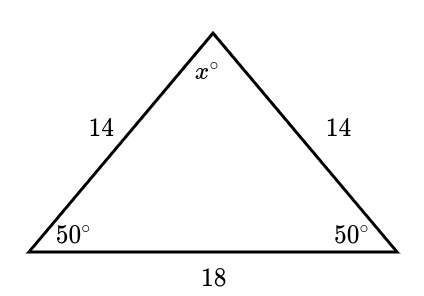
\includegraphics[width=0.9\linewidth]{../images/findangle01a.png}
                \caption{}
                \label{fig:findangle01a}
            \end{figure}
        \end{minipage}\hfill
        \begin{minipage}{0.65\textwidth}
            Dado que tiene dos lados congruentes (aquellos cuya longitud es 14), el triángulo es isósceles. Los ángulos opuestos a los lados congruentes también son congruentes, por lo que el ángulo sin etiqueta mide 50$^\circ$ (Ver Figura \ref{fig:findangle01a}).
            Los tres ángulos en un triángulo suman 180$^\circ$. Podemos escribir este enunciado como una ecuación:
            \[x^\circ + 50^\circ + 50^\circ = 180^\circ \]
            \[\therefore x^\circ = 180^\circ - 50^\circ - 50^\circ = 80^\circ\]
        \end{minipage}
    \end{solutionbox}
\end{minipage}